\section{Results}
\label{results}
In this section we presented both the objective and the subjective results obtained.

\subsection{Objective Results}
\label{results_objective}
Table \ref{table:results_no_ext_f0_glott} shows the objective scores obtained for the synthetic speech of the GlottHMM-based system without using the external $F_{0}$ in the feature extraction.
%
The clean samples have been synthesized with the clean configuration while in all the noisy cases the noise reduction configuration was used. 

On the other hand, in Table \ref{table:results_ext_f0_glott} the results for all the noisy cases adapted using the external $F_{0}$ are presented.
%
In this case, there is no clean row, as the $F_{0}$ is calculated from the clean samples.
%
All the adaptations where done with the noise reduction configuration.

As it can be seen, there are no significant differences between both approaches, what could lead us to think we can use either of the approaches and obtain the same results.
%
However, when listening to the synthesized audio samples it becomes pretty clear that when not using an external $F_{0}$ there is a huge quality drop.
%
Therefore, not using an external $F_{0}$ is been rejected from this point on.



\begin{table}[!htb]
\begin{center}
\begin{tabular}{c c | c | c}
Noise & SNR & fwS & MCD\\
\midrule
\midrule
Clean & - & 9.0 & 1.8\\
\midrule
\multirow{3}{*}{Babble} & 20 & 10.6 & 3.0\\
 & 10 & 7.5 & 2.7\\
 & 5 & 6.3 & 2.6\\
\midrule
\multirow{2}{*}{Factory} & 10 & 6.8 & 3.0\\
 & 5 & 5.3 & 3.2\\
\midrule
Machine gun & 0 & 9.3 & 2.7\\
\midrule
\midrule
\multirow{2}{*}{Enhanced} & 20 & 10.8 & 3.0\\
\multirow{2}{*}{Babble} & 10 & 8.4 & 2.8\\
& 5 & 6.9 & 2.8\\
\midrule
Enhanced & 10 & 8.7 & 3.2\\
Factory & 5 & 7 & 3.3\\
\bottomrule
\end{tabular}
\caption{Objective scores for the adapted test data using the $F_{0}$ calculated for each case with the GlottHMM-based system}
\label{table:results_no_ext_f0_glott}
\end{center}
\end{table}

In Table \ref{table:comp_adapt_results} the comparison between the GlottHMM and STRAIGHT systems can be evaluated through the objective scores.
%
The above result in the clean row is obtained with the clean configuration of GlottHMM, while the one below is obtained using the noise reduction configuration.
%
The contradictory results in the case of the GlottHMM-based system still happening: when SNR shows an improvement the MCD shows a quality decrease.
%
Also, the GlottHMM-based system is found to suffer more degradation under severe noise conditions than the STRAIGHT one.
%
We can spot that the noise reduction system makes the MCD values to increase, as so as the SNR values, giving the contradictory results previously seen.

\begin{table}[!htb]
\begin{center}
\begin{tabular}{c c | c | c}
Noise & SNR & fwS & MCD\\
\midrule
\midrule
\multirow{3}{*}{Babble} & 20 & 10.7 & 3.0\\
 & 10 & 7.6 & 2.7\\
 & 5 & 6.4 & 2.7\\
\midrule
\multirow{2}{*}{Factory} & 10 & 6.9 & 2.9\\
 & 5 & 5.5 & 3.2\\
\midrule
Machine gun & 0 & 9.4 & 2.7\\
\midrule
\midrule
\multirow{2}{*}{Enhanced} & 20 & 10.6 & 3.0\\
\multirow{2}{*}{Babble} & 10 & 8.4 & 2.8\\
& 5 & 6.8 & 2.7\\
\midrule
Enhanced & 10 & 8.7 & 3.2\\
Factory & 5 & 7.1 & 3.3\\
\bottomrule
\end{tabular}
\caption{Objective scores for the adapted test data using an external in the feature extraction $F_{0}$ calculated from the clean data with the GlottHMM-based system}
\label{table:results_ext_f0_glott}
\end{center}
\end{table}

\begin{table}[htb]
\begin{centering}
\begin{tabular}{c c|c c|c c}
	 & & \multicolumn{2}{c|}{Adapted} & \multicolumn{2}{c}{Adapted}\\
	 & & \multicolumn{2}{c|}{GlotHMM} & \multicolumn{2}{c}{STRAIGHT}\\
	 & & \multicolumn{2}{c|}{synthesized} & \multicolumn{2}{c}{synthesized}\\
	 & & \multicolumn{2}{c|}{test data} & \multicolumn{2}{c}{test data}\\
	Noise & SNR & fwS & MCD & fwS & MCD\\
	\midrule
	\midrule
	\multirow{2}{*}{Clean} & \multirow{2}{*}{-} & 9.0 & 1.8 & \multirow{2}{*}{7.5} & \multirow{2}{*}{2.1}\\
	 & & 10.6 & 2.9 & & \\	
	\midrule
	\multirow{3}{*}{Babble} & 20 & 10.7 & 3 & 8.0 & 2.0\\
	 & 10 & 7.6 & 2.7 & 7.5 & 2.1\\
	 & 5 & 6.4 & 2.7 & 7.3 & 2.2\\
	\midrule
	\midrule
	\multirow{2}{*}{Enhanced} & 20 & 10.6 & 3.0 & 8.0 & 2.0\\
	\multirow{2}{*}{Babble} & 10 & 8.4 & 2.8 & 7.5 & 2.1\\
	 & 5 & 6.8 & 2.7 & 7.3 & 2.2\\
	\bottomrule
\end{tabular}
\caption{Objective scores comparing GlottHMM and STRAIGHT}
\label{table:comp_adapt_results}
\end{centering}
\end{table}

\subsection{Subjective Results}
\label{results_subjective}
In the listening test two male voices were evaluated for different vocoders adaptation and different GlottHMM configurations by 32 native speakers using a web-based test.

Two different AB test were carried out. 
%
The first one, 

\begin{figure}[!htb]
  \begin{centering}
  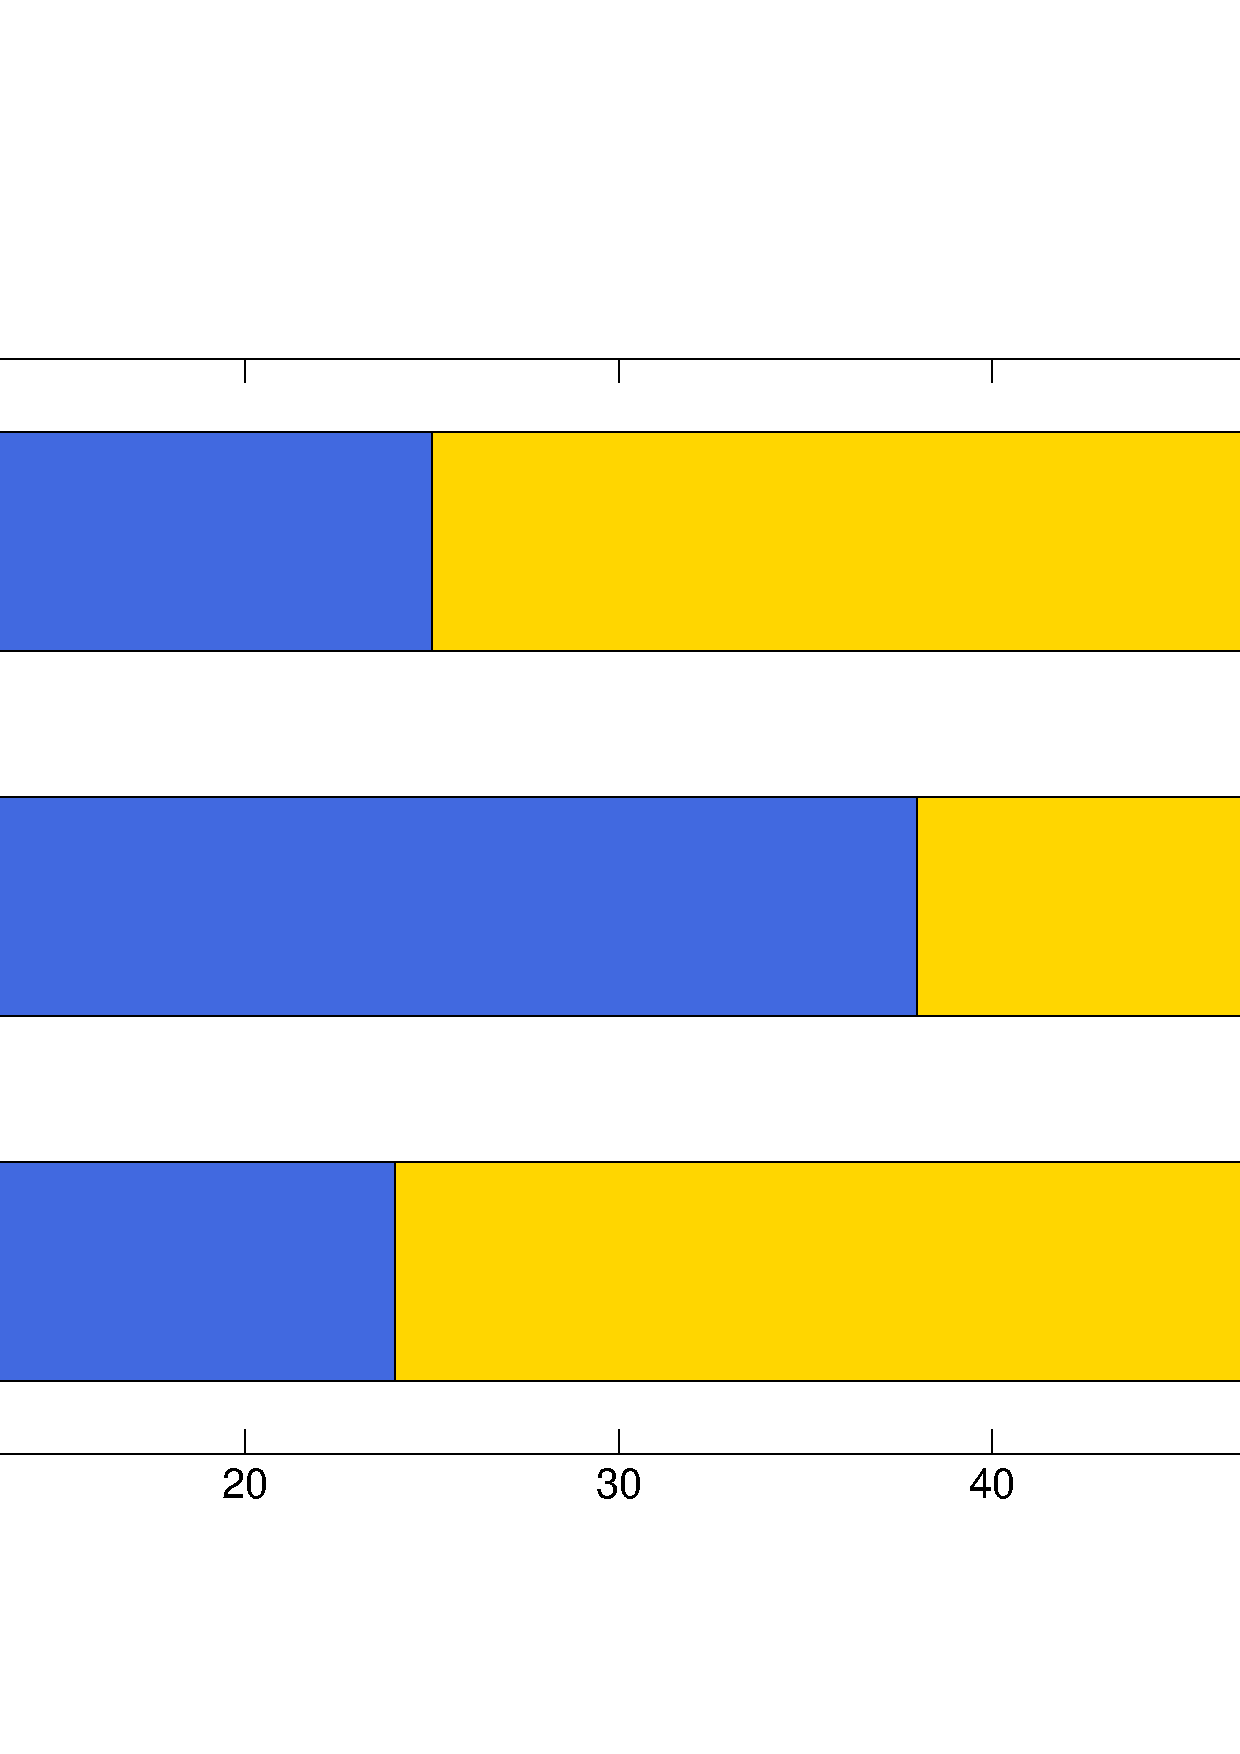
\includegraphics[width=\textwidth]{images/glott_vs_glott.pdf}
  \caption{}
  \label{fig:glott_vs_glott}
  \end{centering}
\end{figure}

\begin{figure}[!htb]
  \begin{centering}
  \includegraphics[width=\textwidth]{images/glott_vs_st.pdf}
  \caption{}
  \label{fig:glott_vs_st}
  \end{centering}
\end{figure}

\begin{figure}[!htb]
  \begin{centering}
  \includegraphics[width=\textwidth]{images/all_subjective_test_quality.pdf}
  \caption{}
  \label{fig:mos_scores}
  \end{centering}
\end{figure}